\section{Experiments}

\subsection{Monk Results}

For all MONK problems, we adopted one-hot encoding for representing the inputs, so we used neural networks with $17$ input units. We used $1$ hidden layer with $4$ units for the first two problems and $5$ for the last one. For what concerns activation functions, we used \texttt{tanh} for the hidden layer, and \texttt{sigmoid} for the output layer to get outputs in the $[0, 1]$ range.

We chose \texttt{MSE} as the loss function over the "raw" output of the \texttt{sigmoid} in order to have differentiability, and instead for predictions every input is classified as $1$ if the output of the \texttt{sigmoid} is $\ge 0.5$ and $0$ otherwise.

We used mini-batch gradient descent with $\texttt{batch\_size} = 4$ for the first Monk problem and $2$ for the others, and L2 regularization for Monk3.

Our choice of hyper-parameters is shown in \cref{fig:hyper} below, along with the performance averaged over $5$ different runs to avoid the bias due to weights initialization.

For MONK 3, we observed that without regularization there is overfitting in all the $5$ runs, so we needed to introduce a regularization penalty (L2) of $10^{-4}$.

\begin{table}[htb]
    \centering
    \begin{tabular}{|c|c|c|c|c|}
        \hline 
        Task & $\eta$ & $\lambda$ & MSE (train/test) & Accuracy (train/test) \\ \hline
        MONK 1 & 0.5 & 0 & 0.00084/0.00128  & 100\%/100\% \\ \hline
        MONK 2 & 0.2 & 0 & 0.00062/0.00073 & 100\%/100\% \\ \hline
        MONK 3 (no regularization) & 0.02 & 0 & 0.05048/0.04236 & 94.26\%/96.06\% \\ \hline
        MONK 3 (regularization) & 0.02 & $10^{-4}$ & 0.06781/0.05215 & 93.44\%/97.22\% \\ \hline
    \end{tabular}
    \caption{Performance results on MONK datasets}
    \label{fig:hyper}
\end{table}

\begin{figure}
    \centering
    \subfloat[Loss]{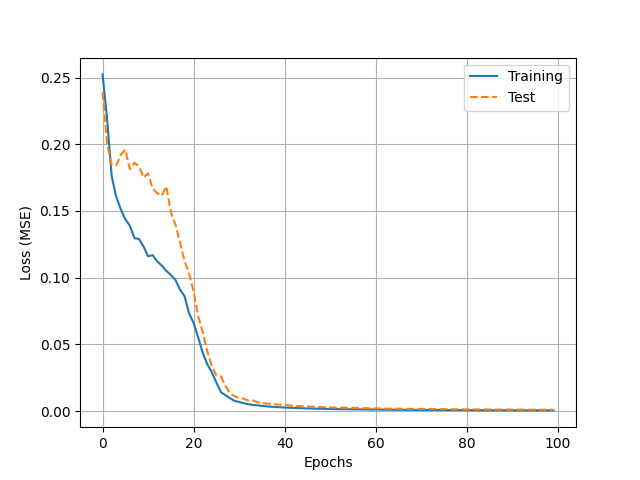
\includegraphics[width=0.5\textwidth]{../results/monks/monk1_losses.png}}
    \subfloat[Accuracy]{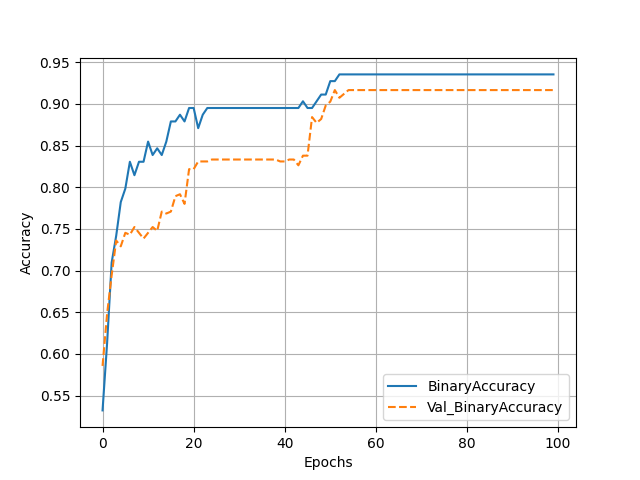
\includegraphics[width=0.5\textwidth]{../results/monks/monk1_accuracy.png}}
    \caption{Loss and accuracy of MONK 1}
    \label{fig:monk1}
\end{figure}

\begin{figure}
    \centering
    \subfloat[Loss]{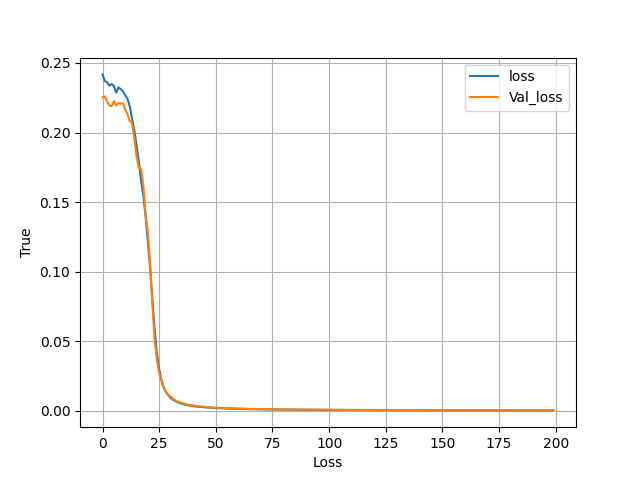
\includegraphics[width=0.5\textwidth]{../results/monks/monk2_losses.png}}
    \subfloat[Accuracy]{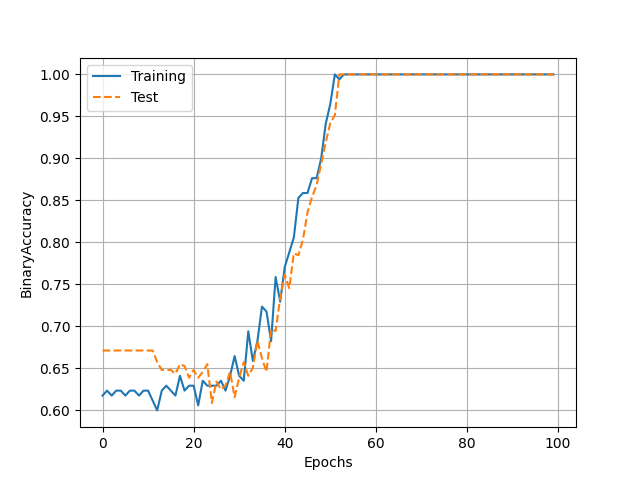
\includegraphics[width=0.5\textwidth]{../results/monks/monk2_accuracy.png}}
    \caption{Loss and accuracy of MONK 2}
    \label{fig:monk2}
\end{figure}

\begin{figure}
    \centering
    \subfloat[Loss]{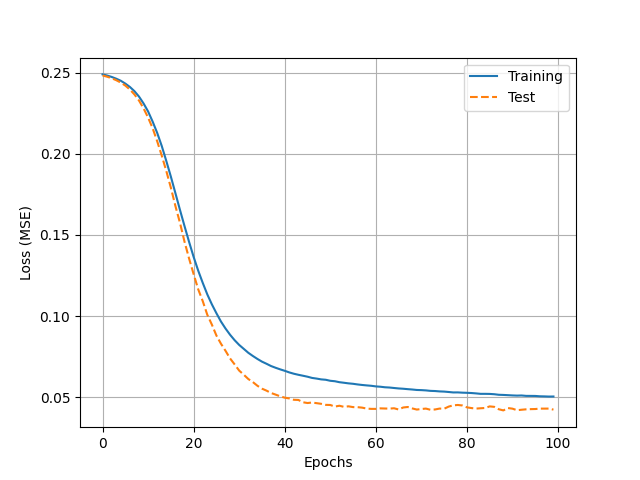
\includegraphics[width=0.5\textwidth]{../results/monks/monk3_noregularization_losses.png}}
    \subfloat[Accuracy]{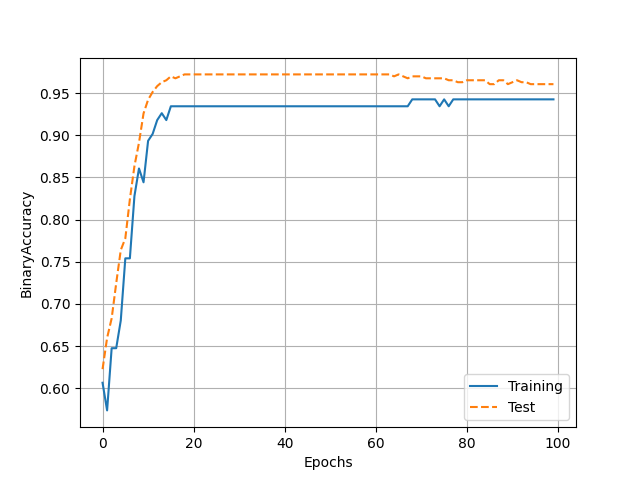
\includegraphics[width=0.5\textwidth]{../results/monks/monk3_noregularization_accuracy.png}}
    \caption{Loss and accuracy of MONK 3 without regularization.}
    \label{fig:monk3_no_reg}
\end{figure}

\begin{figure}
    \centering
    \subfloat[Loss]{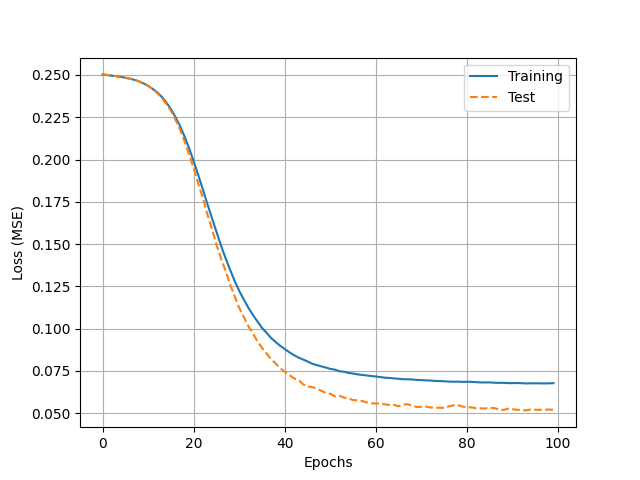
\includegraphics[width=0.5\textwidth]{../results/monks/monk3_regularization_losses.png}}
    \subfloat[Accuracy]{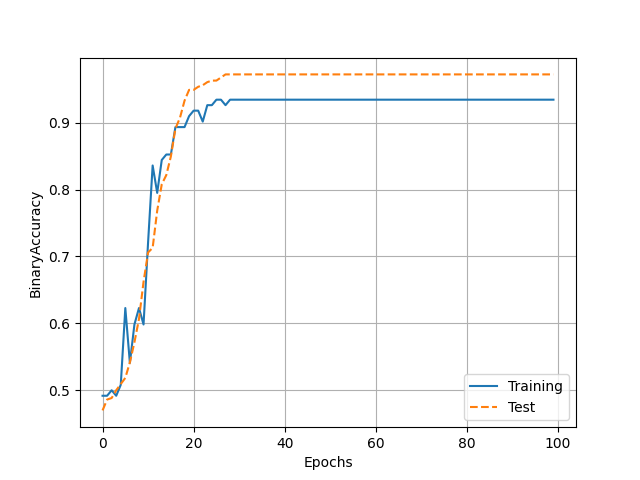
\includegraphics[width=0.5\textwidth]{../results/monks/monk3_regularization_accuracy.png}}
    \caption{Loss and accuracy of MONK 3 with L2 regularization.}
    \label{fig:monk3}
\end{figure}

\subsection{Cup results}

At the beginning, we split the CUP dataset in \textbf{Development Set} ($90\%$ of the dataset, $1342$ records) and in  \textbf{Internal Test Set} ($10\%$ of the dataset, $150$ records). The aim of the first dataset was to be used for subsequent training-validation splits for model selection and training, while the second one was used for testing. After that, we ran several coarse-grained Grid Searches using 3-fold cross validation on the Development Set and finally a fine-grained Grid Search over refined intervals for the hyperparameters using 4-fold cross validation on the Development Set.

\subsubsection{Preliminary trials}

We initially ran several experiments using \texttt{EarlyStopping} \cite{haykin2009neural} for figuring out the order of magnitude of the maximum number of epochs for which there is still significant improvement; our \texttt{EarlyStopping} was configured such that it considered $10^{-4}$ or $10^{-5}$ to be minimum difference on Validation MEE to consider it an improvement. They revealed us that in many cases the improvement on training set was at most of order of $10^-4$ between epoch $500$ and $1000$, while the loss and MEE on the validation set either remained stable or started to grow. We then decided to put $500$ as the maximum number of epochs, also to limit possible overfitting since we wanted to use k-fold cross-validation for our model selection. We similarly ran other test to discard some parameters and speed up the grid search. 

After that, we discarded learning rates of order $ \geq 10^-1$ or $\leq 10^-4$, since they showed worse results than $10^-2$ and $10^-3$, and we selected $256$ aas minibatch size, since it appeared to us the best compromise between the capability of minibatch algorithm to reach better results than batch ones, the speed of training phases and the stability and smoothness of the learning curves. Similarly, for L2 regularization lambda we have discarded values of order $\ge 10^{-3}$ or $\le 10^{-8}$.

We also tested different network architectures, and we noticed that the ones with two hidden layers performed better then the ones with a single hidden layer. Moreover, architectures with three hidden layers did not perform better than the former, so we decided to focus on architectures with 2 hidden layers.

Finally, we discarded small ranges for weights initialization (e.g. uniform distribution in $[-0.1, 0.1]$), since they performed worse than higher ones,
and we fixed uniform distribution in the range $[-0.7, 0.7]$ for weights initialization.

\subsubsection{Grid search}

At first, we conducted a coarse-grained Grid Search over $1296$ possible configurations with large steps for hyperparameters whose purpose was to figure out best intervals or values for the hyperparameters inside the possible values or orders of magnitude we selected after preliminary trials. This first Grid Search uses \textbf{3-fold cross validation} on the Development Set for evaluating configurations and was performed exhaustively among the following hyperparameters:

\begin{itemize}
    \item \textbf{Architecture (hidden units)}: {$32-16$, $16-16$, $16-8$};
    \item \textbf{Activation functions (for hidden layers)}: {\texttt{tanh-tanh}, \texttt{tanh-sigmoid}, \texttt{sigmoid-tanh}, \texttt{sigmoid-sigmoid}};
    \item \textbf{(Initial) learning rate ($\eta_0$)}: {$0.01$, $0.005$, $0.001$};
    \item \textbf{Momentum}: {$0$, $0.4$, $0.8$};
    \item \textbf{L2 Regularization Lambda}: {$10^{-4}$, $10^{-5}$, $10^{-6}$, $10^{-7}$};
    \item \textbf{Learning Rate Decay}: {no decay, linear decay up to $0.1 \cdot \eta_0$, linear decay up to $0.01 \cdot \eta_0$};
\end{itemize}

where with "linear decay up to $\eta_1$" we mean that if the number of epochs is $N$ (in our case $N = 500$), at the epoch $0 \leq x \le N$ (counting from $0$) we had a learning rate of $\eta(x) := \left(1 - \frac{x}{N}\right)\eta_0 + \frac{x}{N} \eta_1$. We have used a "relative" value of $\frac{\eta_0}{\eta_1}$ rather than a fixed constant $\eta_1$ in order to be sure that it always holds $\eta_1 \leq \eta_0$ (otherwise we could have got $\eta_0 = \eta_1 = 10^{-3}$ for instance).

We decided to use k-fold cross validation right from the beginning since we wanted to get less biased results with respect to both weights initialization and training-validation splits.

After that first search, we ranked all the configurations according to their average validation MEE over all the folds and we assigned a score to each hyperparameter calculated as following: if the total number of configurations is $N$ and a given value $x$ for a given hyperparameter $H$ appears in positions $i_1 \leq ... \leq i_k \leq N$, its score is: $\sum_{j=1}^{k}{(N - i_j)}$. We used this score as an indicative heuristics for choosing activation functions and for fine-tuning initial learning rate and momentum. For L2 lambda and learning rate decay, there was no clear "winner", so we ran another coarse-grained Grid Search with approximately the already selected values for the above-mentioned hyperparameters and we fine-tuned L2 lambda, while for decay having $10^{-1}$ or $10^{-2}$ seemed ininfluent, so we kept only the first one.

After that, we performed another exhaustive finer-grained Grid Search with \textbf{4-fold cross validation} over all the $2880$ combinations of the following hyperparameters:
\begin{itemize}
    \item \textbf{Architecture (hidden units)}: $\{32-16, 16-16, 16-8\}$;
    \item \textbf{Activation functions (for hidden layers)}: {tanh-tanh, tanh-sigmoid};
    \item \textbf{(Initial) learning rate ($\eta_0$)}: $\{0.01, 0.009, 0.008, 0.007, 0.006, 0.005\}$;
    \item \textbf{Momentum}: $\{0.4, 0.5, 0.6, 0.7, 0.8\}$;
    \item \textbf{L2 Regularization Lambda}: $\{10^-5, 8\cdot10^-6, 6\cdot10^-6, 4\cdot10^-6, 2\cdot10^-6, 10^-6, 8\cdot10^-7, 6\cdot10^-7\}$;
    \item \textbf{Learning Rate Decay}: {no decay, linear decay up to $0.1 \cdot \eta_0$}.
\end{itemize}
As before, we ranked all the configurations according to their average Validation MEE over all the folds and we finally selected the best model as our final model, trained it on the whole development set and used it for predicting outputs for the blind test set.

Table \ref{tab:heuristics} shows some of the heuristics values after the coarse-grained Grid Searches.

\begin{table}[htb]
    \centering
    \resizebox{0.9\textwidth}{!}{
    \begin{tabular}{|c|c|}
        \hline
        Hyperparameter & Values \\ \hline
        Activation & $\texttt{tanh-tanh}: 247924$, $\texttt{tanh-sigmoid}: 225057$ \\ \hline
        Activation (2nd row) & $\texttt{sigmoid-tanh}: 198399$, $\texttt{sigmoid-sigmoid}: 169076$ \\ \hline
        Learning rate & $0.01: 379687$, $0.005: 324272$, $0.001: 136497$ \\ \hline
        Momentum & $0.8: 373121$, $0.4: 261535$, $0.0: 205800$ \\ \hline
        Lambda (1st search) & $10^{-4}: 151572$, $10^{-5}: 228108$, $10^{-6}: 230144$, $10^{-7}: 230632$ \\ \hline
        Lambda (2nd search) & $10^{-5}: 6101$, $5\cdot10^{-6}: 5812$, $10^{-6}: 5486$, $5\cdot10^{-7}: 5985$, $10^{-7}: 5536$ \\ \hline
        Decay & no decay: $330805$, linear $0.01$: $244885$, linear $0.1$: $264766$ \\ \hline
    \end{tabular}
    }
    \caption{Heuristic values for some hyperparameters.}
    \label{tab:heuristics}
\end{table}

\subsubsection{Grid Search Results}
Table \ref{table:grid_search_results} reports the hyperparameters values and the average training, validation and test errors (MEE) over all the 4 folds of the 8 most performant configurations after the fine-grained Grid Search.

\begin{table}[htb]
    \centering
    \resizebox{\textwidth}{!}{
    \begin{tabular}{|c|c|c|c|c|c|c|c|c|}
        \hline
        Architecture & Activation & Learning Rate & Momentum & Lambda & Decay & Error TR & Error VL & Error TS \\ \hline
        $32-16$ & \texttt{tanh-tanh} & $0.005$ & $0.8$ & $6\cdot10^-6$ & linear $0.1$ & $1.2680$ & $1.4246$ & $1.3857$ \\ \hline
        $32-16$ & \texttt{tanh-tanh} & $0.009$ & $0.8$ & $6\cdot10^-7$ & linear $0.1$ & $1.2338$ & $1.4268$ & $1.4836$ \\ \hline
        $16-16$ & \texttt{tanh-tanh} & $0.008$ & $0.7$ & $2\cdot10^-6$ & no decay & $1.2490$ & $1.4269$ & $1.3950$ \\ \hline
        $32-16$ & \texttt{tanh-tanh} & $0.006$ & $0.8$ & $6\cdot10^-6$ & linear $0.1$ & $1.2289$ & $1.4276$ & $1.4281$ \\ \hline
        $16-16$ & \texttt{tanh-tanh} & $0.008$ & $0.8$ & $10^{-5}$ & linear $0.1$ & $1.2852$ & $1.4301$ & $1.3936$ \\ \hline
        $16-16$ & \texttt{tanh-tanh} & $0.009$ & $0.7$ & $4\cdot10^{-6}$ & linear $0.1$ & $1.2829$ & $1.4304$ & $1.4199$ \\ \hline
        $32-16$ & \texttt{tanh-tanh} & $0.009$ & $0.8$ & $6\cdot10^{-6}$ & linear $0.1$ & $1.2134$ & $1.4305$ & $1.4460$ \\ \hline
        $32-16$ & \texttt{tanh-tanh} & $0.006$ & $0.6$ & $8\cdot10^{-6}$ & no decay & $1.2400$ & $1.4318$ & $1.4704$ \\ \hline
    \end{tabular}
    }
    \caption{Hyperparameters and average training, validation and test error (MEE) of the 8 most performant configurations after last grid search}
    \label{table:grid_search_results}
\end{table}

\subsubsection{Computing time and hardware}
The two coarse-grained searches cumulatively took $22$ minutes to complete, while the second one took $57$ minutes using an Intel Core i7-10870H @ 2.00 GHz (16 logical CPUs). We used the \texttt{joblib} library for parallelizing the search by using a pool of $16$ worker processes. The average time requested for a training cycle of a model during the grid search is between $3$ and $5$ seconds for the three different architectures, which is slightly higher than the time needed for a full training of the final chosen model, which is about $3.2$ seconds. For Monk problems, the time required is about $1.2$ seconds for the first problem and $2.1$ for the other two on the same hardware as above, with this difference substantially determined by the different minibatch sizes that we used.

\subsubsection{Chosen model and final discussion}
We finally chose the model that performed best on the validation set, which has the following hyperparameters and training and test errors (MEE) after a full training on the whole development set, which took $3.2$ seconds.

\begin{table}[htb]
    \centering
    \resizebox{\textwidth}{!}{
    \begin{tabular}{|c|c|c|c|c|c|c|c|c|}
        \hline
        Architecture & Activation & Learning Rate & Momentum & Lambda & Decay & Error TR & Error TS \\ \hline
        $32-16$ & \texttt{tanh} & $0.005$ & $0.8$ & $6\cdot10^-6$ & linear $0.1$ & $1.2369$ & $1.4401$ \\ \hline
    \end{tabular}
    }
    \caption{Hyperparameters and training and test error (MEE) of the chosen model after a full training on the whole development set}
    \label{table:final_train_results}
\end{table}
We can see the learning curve for loss (MSE) and MEE in \cref{fig:cup_plots} below.

\begin{figure}[h]
    \centering
    \subfloat[Loss\label{fig:cup_loss}]{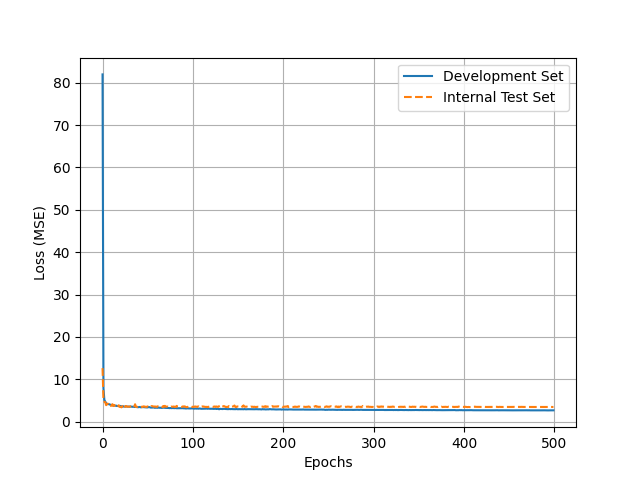
\includegraphics[width=0.55\textwidth]{../results/cup_loss.png}}
    \subfloat[MEE\label{fig:cup_MEE}]{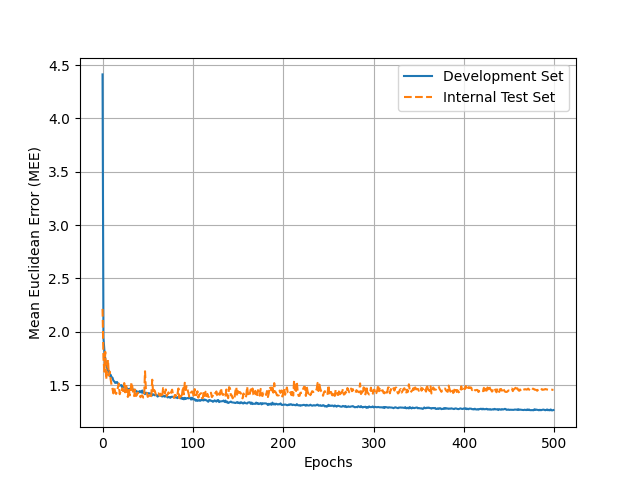
\includegraphics[width=0.55\textwidth]{../results/cup_MEE.png}}
    \caption{Learning curves for CUP network}
    \label{fig:cup_plots}
\end{figure}

We achieved a MEE of $1.4401$ on our internal test set, and we estimate the performance on the blind test set as being near to that value. We have observed that for almost all the cases that we have analyzed both in Grid Searches and in preliminary experiments the validation error is in the range $[1.3, 1.6]$ for all the models with two hidden layers we have tried and for several ones with three hidden layers, regardless of the activation functions and the other hyperparameters. We obtained similar results also with equivalent \texttt{keras} models.

%%% Local Variables:
%%% mode: latex
%%% TeX-master: "report"
%%% End: